\documentclass[12pt,letterpaper]{article}
\usepackage{graphicx,textcomp}
\usepackage{natbib}
\usepackage{setspace}
\usepackage{fullpage}
\usepackage{color}
\usepackage[reqno]{amsmath}
\usepackage{amsthm}
\usepackage{fancyvrb}
\usepackage{amssymb,enumerate}
\usepackage[all]{xy}
\usepackage{endnotes}
\usepackage{lscape}
\newtheorem{com}{Comment}
\usepackage{float}
\usepackage{hyperref}
\newtheorem{lem} {Lemma}
\newtheorem{prop}{Proposition}
\newtheorem{thm}{Theorem}
\newtheorem{defn}{Definition}
\newtheorem{cor}{Corollary}
\newtheorem{obs}{Observation}
\usepackage[compact]{titlesec}
\usepackage{dcolumn}
\usepackage{tikz}
\usetikzlibrary{arrows}
\usepackage{multirow}
\usepackage{xcolor}
\newcolumntype{.}{D{.}{.}{-1}}
\newcolumntype{d}[1]{D{.}{.}{#1}}
\definecolor{light-gray}{gray}{0.65}
\usepackage{url}
\usepackage{listings}
\usepackage{color}

\definecolor{codegreen}{rgb}{0,0.6,0}
\definecolor{codegray}{rgb}{0.5,0.5,0.5}
\definecolor{codepurple}{rgb}{0.58,0,0.82}
\definecolor{backcolour}{rgb}{0.95,0.95,0.92}

\lstdefinestyle{mystyle}{
	backgroundcolor=\color{backcolour},   
	commentstyle=\color{codegreen},
	keywordstyle=\color{magenta},
	numberstyle=\tiny\color{codegray},
	stringstyle=\color{codepurple},
	basicstyle=\footnotesize,
	breakatwhitespace=false,         
	breaklines=true,                 
	captionpos=b,                    
	keepspaces=true,                 
	numbers=left,                    
	numbersep=5pt,                  
	showspaces=false,                
	showstringspaces=false,
	showtabs=false,                  
	tabsize=2
}
\lstset{style=mystyle}
\newcommand{\Sref}[1]{Section~\ref{#1}}
\newtheorem{hyp}{Hypothesis}

\title{Problem Set 1}
\date{Due: October 8, 2026}
\author{William Sarsfield}

\begin{document}
	\maketitle
	
	\section*{Instructions}
	\begin{itemize}
	\item Please show your work! You may lose points by simply writing in the answer. If the problem requires you to execute commands in \texttt{R}, please include the code you used to get your answers. Please also include the \texttt{.R} file that contains your code. If you are not sure if work needs to be shown for a particular problem, please ask.
\item Your homework should be submitted electronically on GitHub.
\item This problem set is due before 23:59 on Thursday October 8, 2026. No late assignments will be accepted.
	\end{itemize}
	
	\vspace{1cm}
	\section*{Question 1: Education}

A school counselor was curious about the average of IQ of the students in her school and took a random sample of 25 students' IQ scores. The following is the data set:\\
\vspace{.5cm}

\lstinputlisting[language=R, firstline=36, lastline=36]{PS01_answers_WS.R}  
\vspace{1cm}

\begin{enumerate}
	\item Find a 90\% confidence interval for the average student IQ in the school (As a hint, you first need the mean and SD to create a CI):\\
	\lstinputlisting[language=R, firstline=37, lastline=47]{PS01_answers_WS.R}  
\begin{verbatim}
Confidence Interval is: 93.95993 102.9201
Mean is: 98.44 
Standard Error is: 2.618575
Critical Value is: 1.710882
 	\end{verbatim}
	\noindent
	To find the 90 percent confidence interval I first calculated the sample mean and standard deviation.  Next I then found the standard error utilising the standard deviation. I then determined  the t-test statistic and found that the confidence interval to be 98.44 ± 4.48. Therefore, I am 90 percent confident that the true population mean is between 93.96 and 102.92
	
	
	\item Next, the school counselor was curious  whether  the average student IQ in her school is higher than the average IQ score (100) among all the schools in the country.\\ 
	
	\noindent Using the same sample, conduct the appropriate hypothesis test with $\alpha=0.05$.
	
		\lstinputlisting[language=R, firstline=48, lastline=56]{PS01_answers_WS.R}  
		
	\begin{verbatim}
	PValue is: 0.7215383 T-test statistic is: -0.5957439
	\end{verbatim}
	\noindent 
	
	The five-step hypothesis test was conducted to determine whether the average IQ score of the students at the counselor's school was higher than the average among all schools in the country. The test produced a p-value  of .7215383 which is much greater than the alpha of .05. Therefore, I cannot reject the null hypothesis that the average IQ in the counselor's school is less than or equal to the country's average.
\end{enumerate}
\newpage

	\section*{Question 2: Political Economy}

\noindent Researchers are curious about what affects the amount of money communities spend on addressing homelessness. The following variables constitute our data set about social welfare expenditures in the USA. \\
\vspace{.5cm}

\begin{tabular}{r|l}
	\texttt{State} &\emph{50 states in US} \\
	\texttt{Y} & \emph{per capita expenditure on shelters/housing assistance in state}\\
	\texttt{X1} &\emph{per capita personal income in state} \\
	\texttt{X2} &  \emph{Number of residents per 100,000 that are "financially insecure" in state}\\
	\texttt{X3} &  \emph{Number of people per thousand residing in urban areas in state} \\
	\texttt{Region} &  \emph{1=Northeast, 2= North Central, 3= South, 4=West} \\
\end{tabular}

\vspace{.5cm}
\noindent Explore the \texttt{expenditure} data set and import data into \texttt{R}.
\vspace{.5cm}
\lstinputlisting[language=R, firstline=63, lastline=63]{PS01_answers_WS.R}  
\vspace{.5cm}
\begin{itemize}

\item
Please plot the relationships among \emph{Y}, \emph{X1}, \emph{X2}, and \emph{X3}? What are the correlations among them (you just need to describe the graph and the relationships among them)?
\vspace{.5cm}
\lstinputlisting[language=R, firstline=67, lastline=69]{PS01_answers_WS.R}  
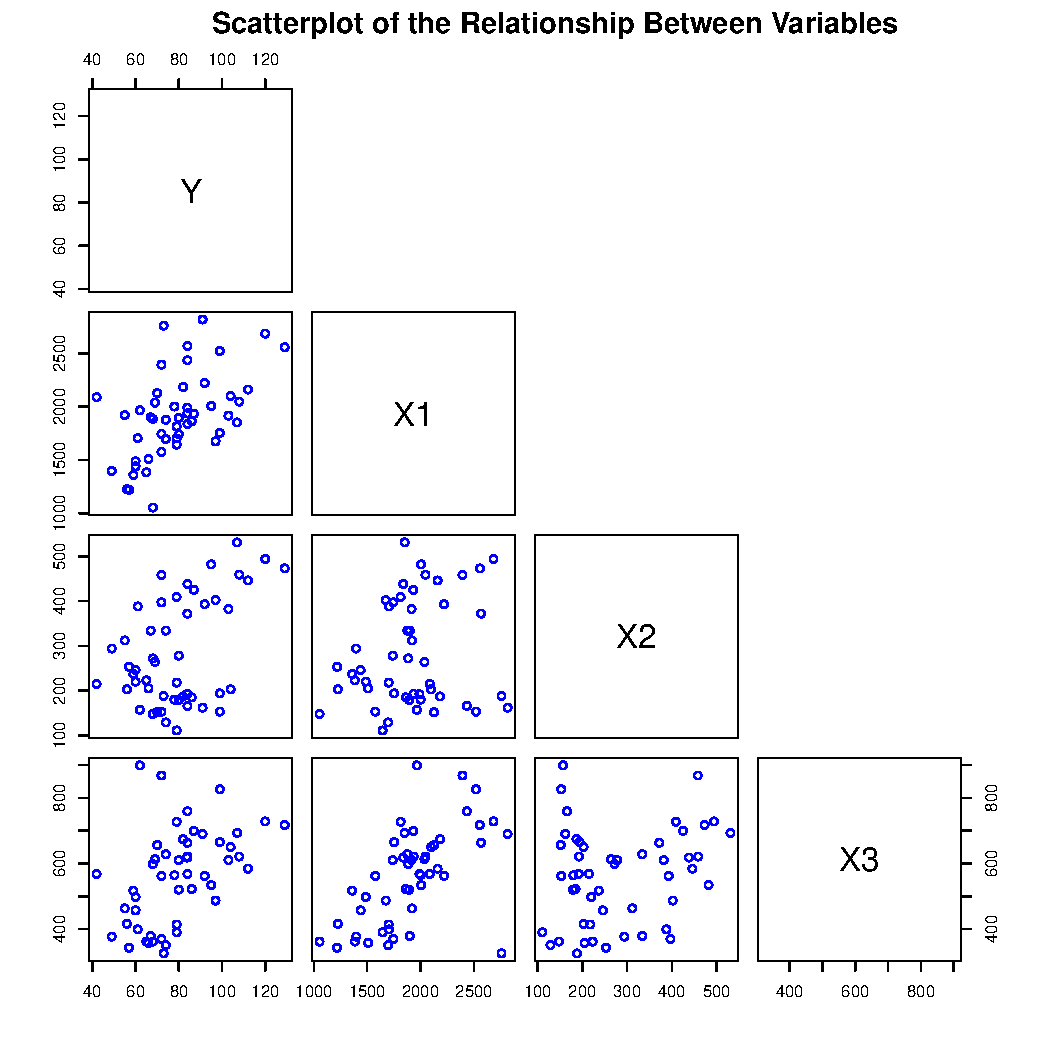
\includegraphics[width=.75\textwidth]{Scatterplot.pdf}
\noindent 

The scatterplots above show the relationship among the four variables. Using these graphs, it is possible to judge the preliminary correlation between the four variables. 
	
	Looking first at  \textit{Y}, its relationship with \textit{X1}  demonstrates a moderately strong positive relationship signalling a positive correlation. This suggests that, on average, as expenditure on shelter use in a state increases, so does per capita personal income. However, for \textit{Y's} relationship with \textit{X2} the two variables appear to be uncorrelated and at best a weak relationship between the two variables. Thus, suggesting that, on average, an increase in a state's  expenditure on shelter and housing on average cannot predict an increase or decrease in the number of residents per 100,000 who are financially insecure. Further, the relationship between \textit{X3} and \textit{Y} appears to have a positive relationship and potential positive correlation. Demonstrating that as the per capita expenditure on shelters and housing increases so will the number of people per thousand residing in urban areas in the state. 
	
	Examining \textit{X1}, its relationship with \textit{X2} appears to have a weak correlation and no discernible association or relationship; thus any increase in the per capita personal income in a state on average would not predict any discernible change in the number of residents per 100,000 who are financially insecure inside of a state. The relationship between \textit{X1} and \textit{X3} demonstrates that the two variables likely have a positive association and have a likely positive correlation, demonstrating that states with higher per capita personal income would, on average, tend to have more people per thousand residing in urban areas in the state. 
	
	For the last relationship between variables \textit{X2} and \textit{X3} appears to show little correlation, with neither a positive nor a negative relationship. Therefore, an increase in the number of residents per 100,000 who are financially insecure does not impact the number of people per thousand residing in urban areas in a state. 
\item
Please plot the relationship between \emph{Y} and \emph{Region}? On average, which region has the highest per capita expenditure on housing assistance?
\vspace{.5cm}
\lstinputlisting[language=R, firstline=77, lastline=82]{PS01_answers_WS.R}  
\noindent \textbf{First} I renamed the variable  Region calling it a new variable "NamedRegions", so that it would be able to be utilised to create an accurate key for the second and third part of Question 2
\lstinputlisting[language=R, firstline=84, lastline=89]{PS01_answers_WS.R}  

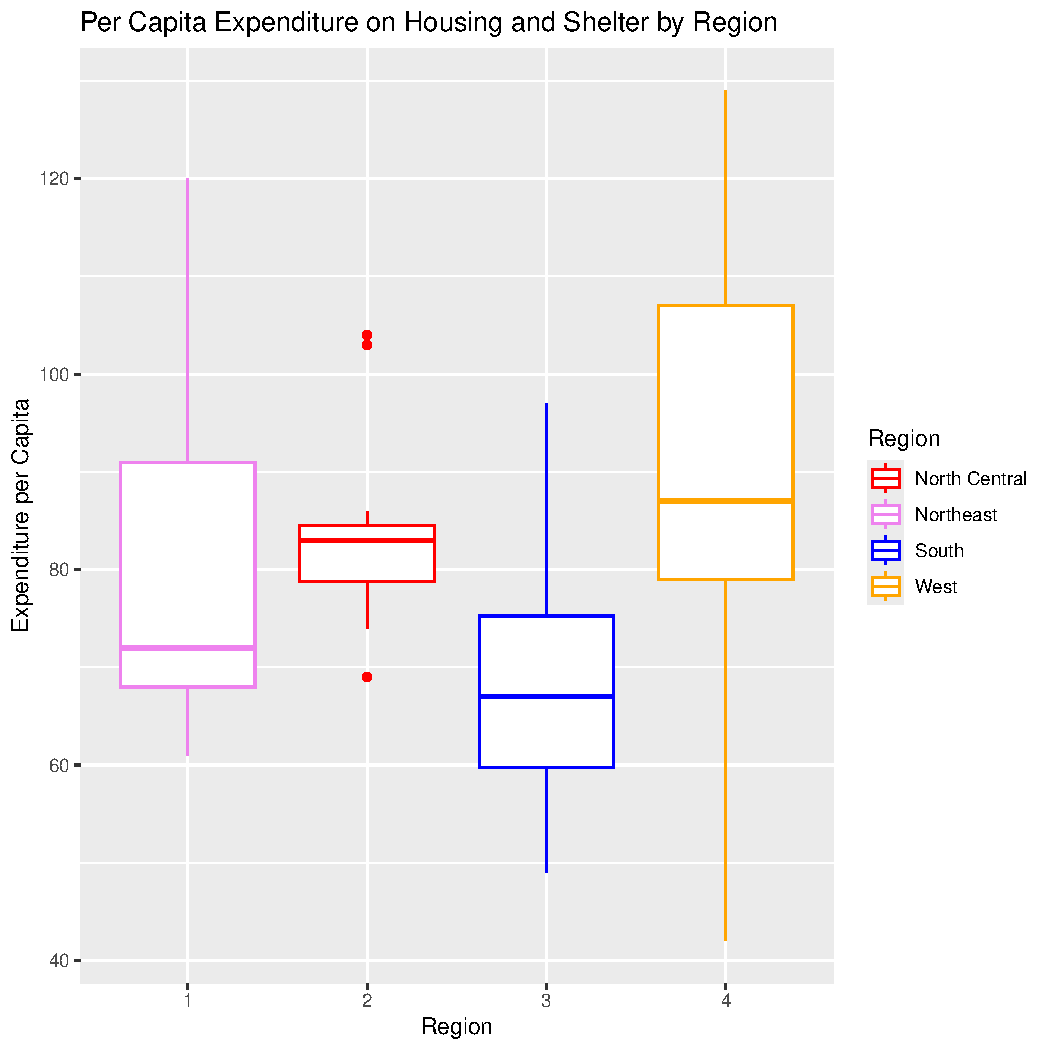
\includegraphics[width=1\textwidth]{Boxplot.pdf}
\noindent

 As demonstrated by the boxplots the West Region has, on average the highest per capita expenditure on housing assistance. The boxplots also demonstrate that the West Region has the widest range of per capita expenditure on housing assistance, and the Northeast has the second-widest range. However, the North Central actually had the second-highest average despite having the lowest IQR.

\item
Please plot the relationship between \emph{Y} and \emph{X1}? Describe this graph and the relationship. Reproduce the above graph including one more variable \emph{Region} and display different regions with different types of symbols and colors.
\lstinputlisting[language=R, firstline=95, lastline=102]{PS01_answers_WS.R}  
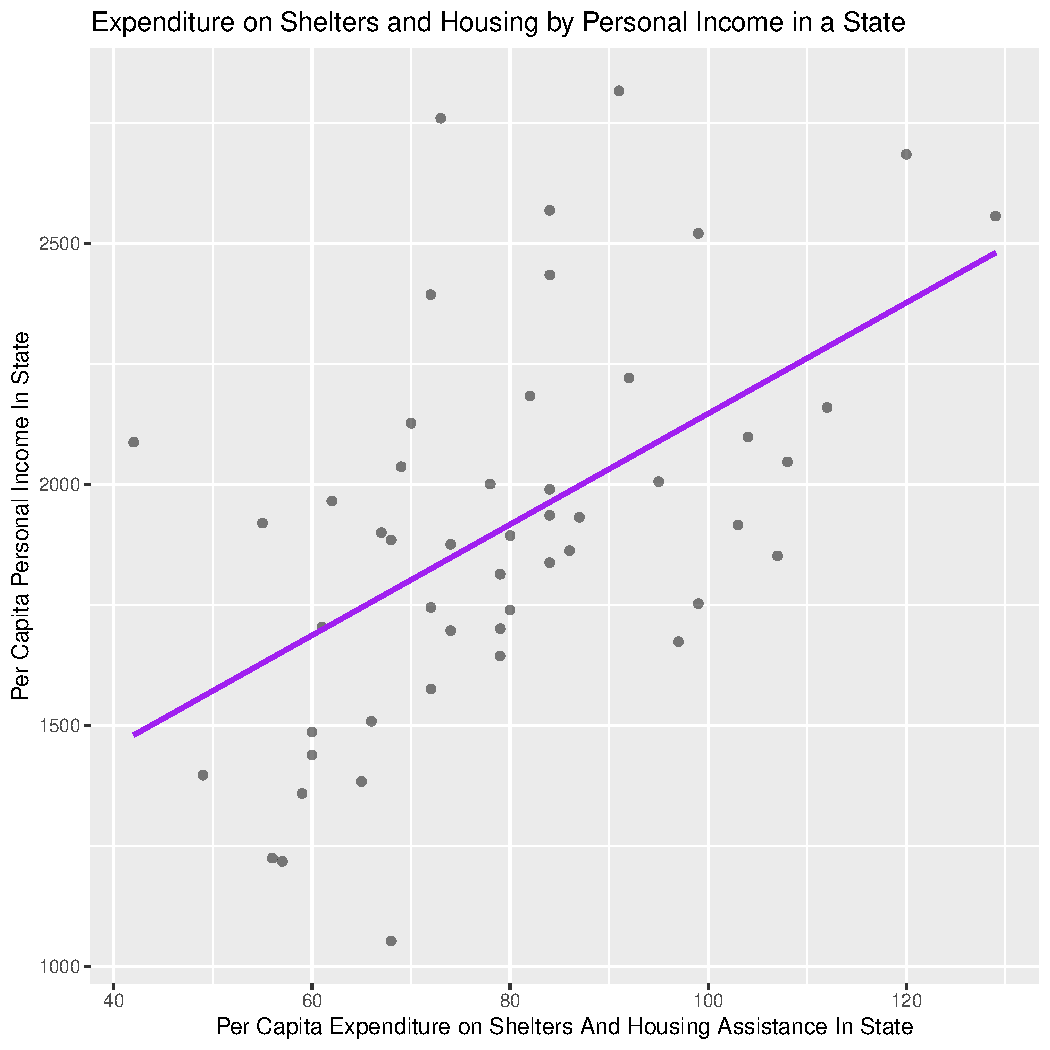
\includegraphics[width=1\textwidth]{Shelter.pdf}
\indent \textbf{First Plot} The relationship between per capita expenditure on shelters and housing assistance in a state and per capita personal income in a state appears linear, as demonstrated by the line of best fit added to the graph showing a projected y-intercept just above 1,400. Overall, this demonstrates that as per capita expenditure on shelters and housing assistance increases, so does, on average, the per capita personal income in the same state, thus demonstrating a positive relationship between the variables.
\lstinputlisting[language=R, firstline=103, lastline=114]{PS01_answers_WS.R}  
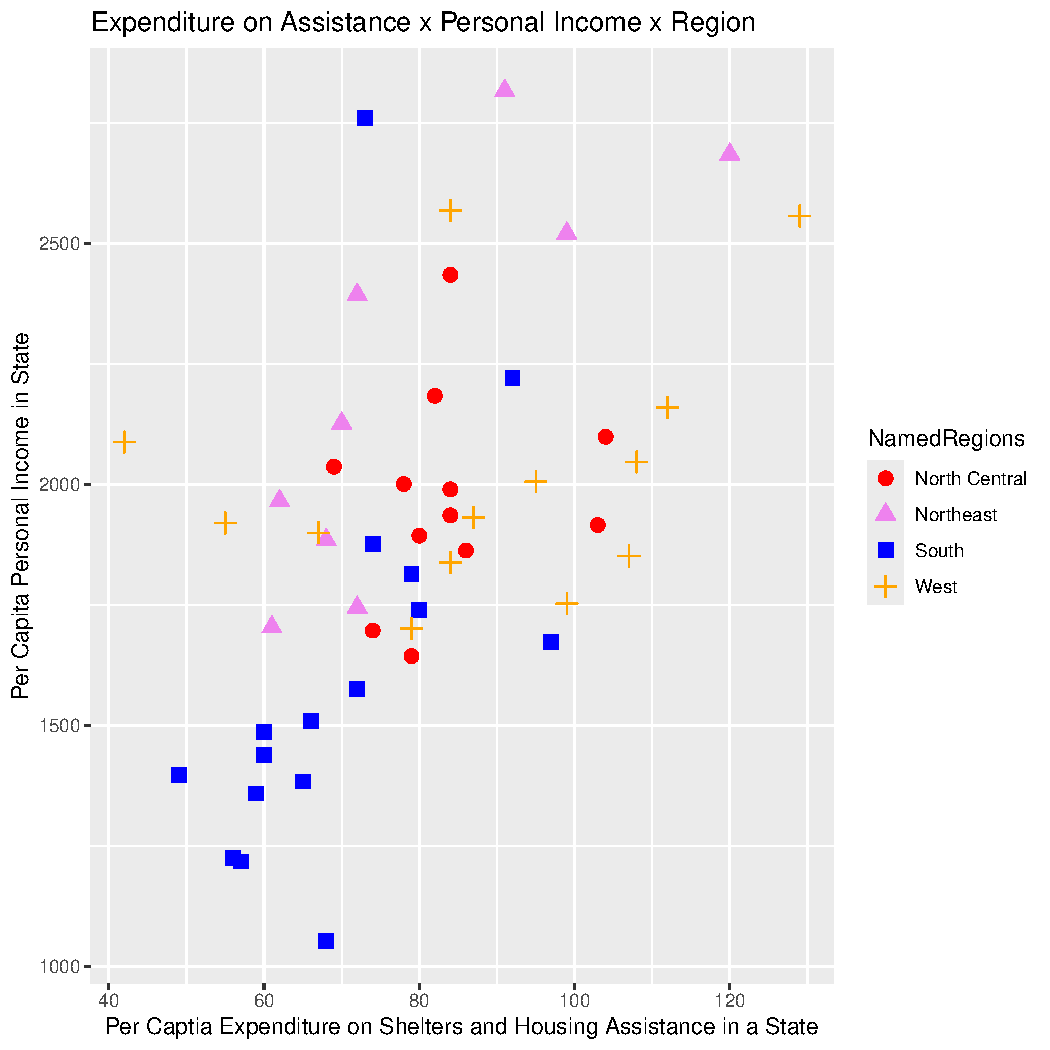
\includegraphics[width=1\textwidth]{ShelterRegion.pdf}
\indent \textbf{Second Plot} Utilising region to differentiate datapoints on the scatterplot shows how  the relationship between per capita expenditure on shelters and housing assistance in a state and per capita personal income in a state differs by region. The South Region is represented by the blue squares and has a clustering of data points at the lower levels of per capita expenditure on housing and shelter and personal income per capita. Thus showing less expenditure and income in the South Region specifically. However, on average, the other regions were more equally dispersed throughout the scatterplot.

\end{itemize}

\end{document}
